\documentclass{beamer}
\usetheme{Boadilla}
\usepackage[utf8]{vietnam}
\usepackage{multirow}
\usepackage{graphicx}
\usepackage{makecell}
\usepackage{adjustbox}

\begin{document}
    % ===== TRANG BÌA =====
    \begin{frame}
        \vspace{-0.3cm}
        \begin{figure}
            \centering
            
\includegraphics[width=0.25\linewidth]{img/Picture1.png}
        \end{figure}
        
        \begin{center}\Large
            \textbf{BÁO CÁO CUỐI KỲ}
        \end{center}
        
        \begin{center}
            \textbf{\underline{MÔN HỌC:} QUẢN TRỊ HỆ THỐNG MẠNG}
        \end{center}
        
        \begin{center}
            \textbf{\underline{Chủ đề:}} TRIỂN KHAI, QUẢN LÝ, CẤU HÌNH PRINTER SERVER
        \end{center}
        
        \begin{center}\small
            \textbf{\textcolor{red}{Sinh viên thực hiện:}}\\
            \vspace{0.1cm}
            \textbf{PHAN TRÍ TÂM - 52300253}\\
            \textbf{HOÀNG HỮU PHÚC - 52300240}\\
            \textbf{NGUYỄN TẤN MẠNH - 52300221}
        \end{center}
        
        \begin{center}
            \textbf{\underline{Ngành:} Mạng máy tính và truyền thông dữ liệu}\\
        \end{center}
    \end{frame}

    % ===== MỤC LỤC =====
    \begin{frame}{Mục lục}
        \tableofcontents
    \end{frame}

    % ===== GIỚI THIỆU =====
    \section{Giới thiệu}
    \begin{frame}{Thông tin dự án}
        \begin{itemize}
            \item \textbf{Tên dự án:} Triển khai Printer Server – Doanh Nghiệp ABC
            \item \textbf{Môn học:} Quản trị Hệ Thống Mạng
            \item \textbf{Ngày hoàn thành:} Tháng 12 năm 2025
            \item \textbf{Công nghệ:} 
                \begin{itemize}
                    \item Windows Server 2019
                    \item PowerShell
                    \item Active Directory
                \end{itemize}
            \item \textbf{Yêu cầu đặc biệt:} Triển khai hoàn toàn qua dòng lệnh – Không dùng GUI
        \end{itemize}
    \end{frame}
    
    \begin{frame}{Bối cảnh doanh nghiệp ABC}
        \textbf{Doanh nghiệp giả định ABC có 3 phòng ban chính:}
        \begin{itemize}
            \item \textbf{Phòng Thiết kế (Design):}
                \begin{itemize}
                    \item In màu chất lượng cao
                    \item Ưu tiên tốc độ
                \end{itemize}
            \item \textbf{Phòng Văn phòng (Office):}
                \begin{itemize}
                    \item In văn bản số lượng lớn
                    \item Tối ưu chi phí
                \end{itemize}
            \item \textbf{Phòng Kế toán (Accounting):}
                \begin{itemize}
                    \item In hóa đơn
                    \item Yêu cầu bảo mật cao
                    \item Ghi log chi tiết
                \end{itemize}
        \end{itemize}
    \end{frame}
    
    \begin{frame}{Mục tiêu hệ thống}
        \begin{itemize}
            \item \textbf{Tự động hóa:} 
                \begin{itemize}
                    \item Triển khai máy in theo phòng ban
                    \item Phân phối qua Group Policy
                \end{itemize}
            \item \textbf{Phân quyền:}
                \begin{itemize}
                    \item Dựa trên Group trong Active Directory
                    \item Mỗi phòng ban chỉ truy cập đúng máy in
                \end{itemize}
            \item \textbf{Giám sát:}
                \begin{itemize}
                    \item Ghi log đầy đủ quá trình in
                    \item Xuất báo cáo thống kê theo User
                \end{itemize}
            \item \textbf{Quản lý:}
                \begin{itemize}
                    \item Tạo Printer Pool để chia tải
                    \item Thiết lập độ ưu tiên cho máy in
                \end{itemize}
        \end{itemize}
    \end{frame}

    % ===== HẠ TẦNG HỆ THỐNG =====
    \section{Hạ tầng hệ thống}
    \begin{frame}{Cấu hình Print Server}
        \begin{table}[ht]
            \centering
            \small
            \begin{tabular}{|l|l|}
            \hline
            \textbf{Thông số} & \textbf{Chi tiết} \\
            \hline
            Hostname & SRV-PRINT \\
            \hline
            HĐH & Windows Server 2019 Datacenter \\
            \hline
            IP Address & 192.168.244.10/24 \\
            \hline
            Gateway & 192.168.244.1 \\
            \hline
            DNS Primary & 192.168.244.10 \\
            \hline
            DNS Secondary & 8.8.8.8 \\
            \hline
            Domain & ABC.local \\
            \hline
            Vai trò & DC + Print Server + DNS + AD DS \\
            \hline
            Nền tảng & VMware Workstation Pro \\
            \hline
            \end{tabular}
        \end{table}
    \end{frame}
    \begin{frame}{Sơ đồ kiến trúc hệ thống}
        \begin{figure}
            \centering
            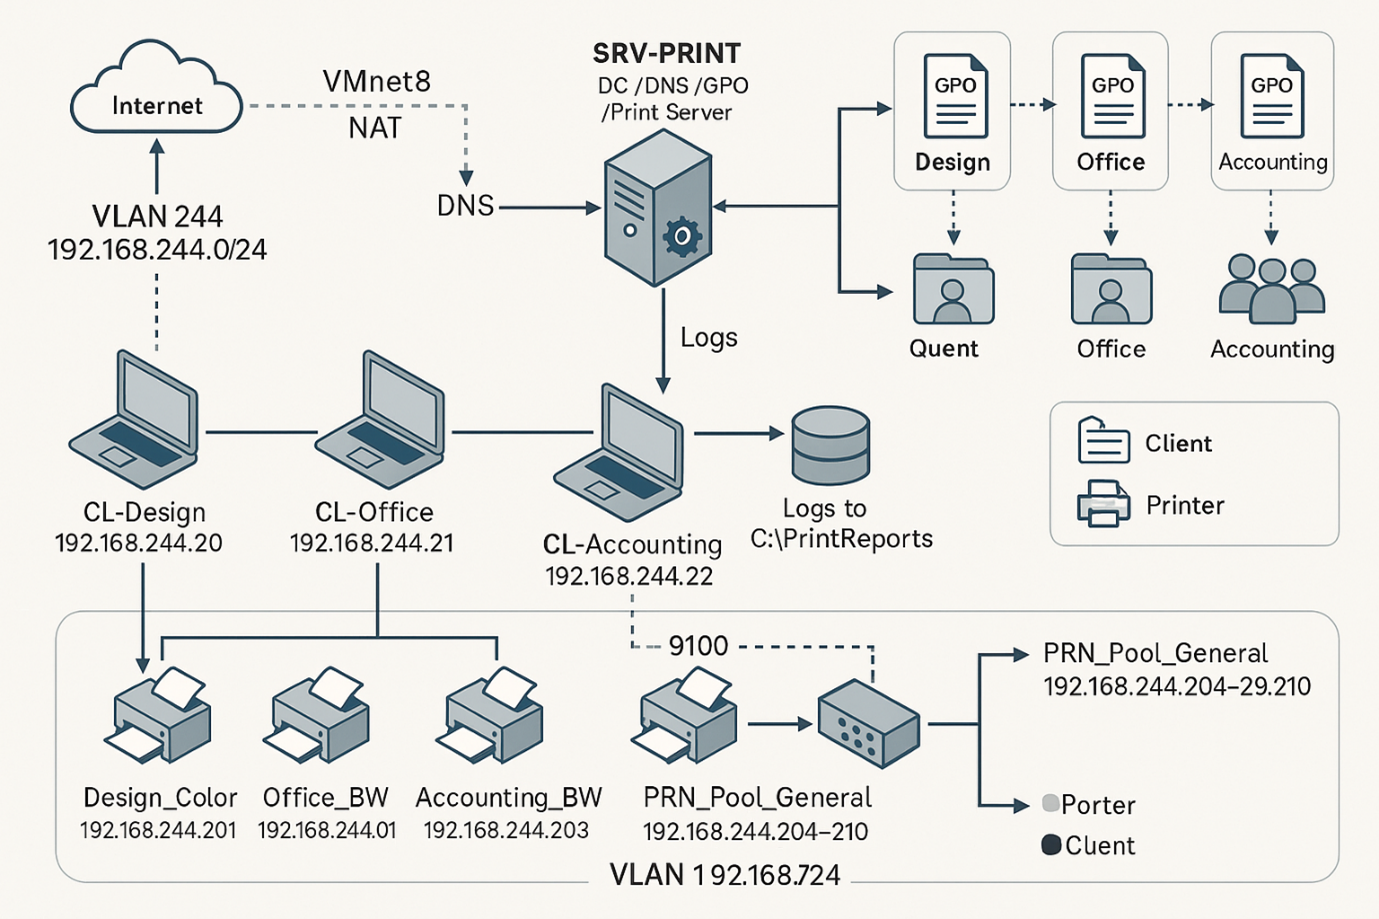
\includegraphics[width=0.85\linewidth]{img/a.png}
            \caption{Sơ đồ cấu trúc tổng thể hệ thống Printer Server}
        \end{figure}
    \end{frame}

    \begin{frame}{Sơ đồ kiến trúc hệ thống}
        \textbf{Các thành phần chính:}
        \begin{itemize}
            \item \textbf{1 máy chủ Windows Server 2019:}
                \begin{itemize}
                    \item Print Server, AD DS, DNS
                    \item Domain: ABC.local
                \end{itemize}
            \item \textbf{3 máy trạm Windows 8.1:}
                \begin{itemize}
                    \item user\_design (Phòng Thiết kế)
                    \item user\_office (Phòng Văn phòng)
                    \item user\_accounting (Phòng Kế toán)
                \end{itemize}
            \item \textbf{10 máy in vật lý/ảo:}
                \begin{itemize}
                    \item Dải IP: 192.168.244.201 – 192.168.244.210
                    \item Bao gồm máy in màu, trắng đen và hoá đơn
                \end{itemize}
        \end{itemize}
    \end{frame}
    \begin{frame}{Sơ đồ hoạt động}
        \begin{figure}
            \centering
            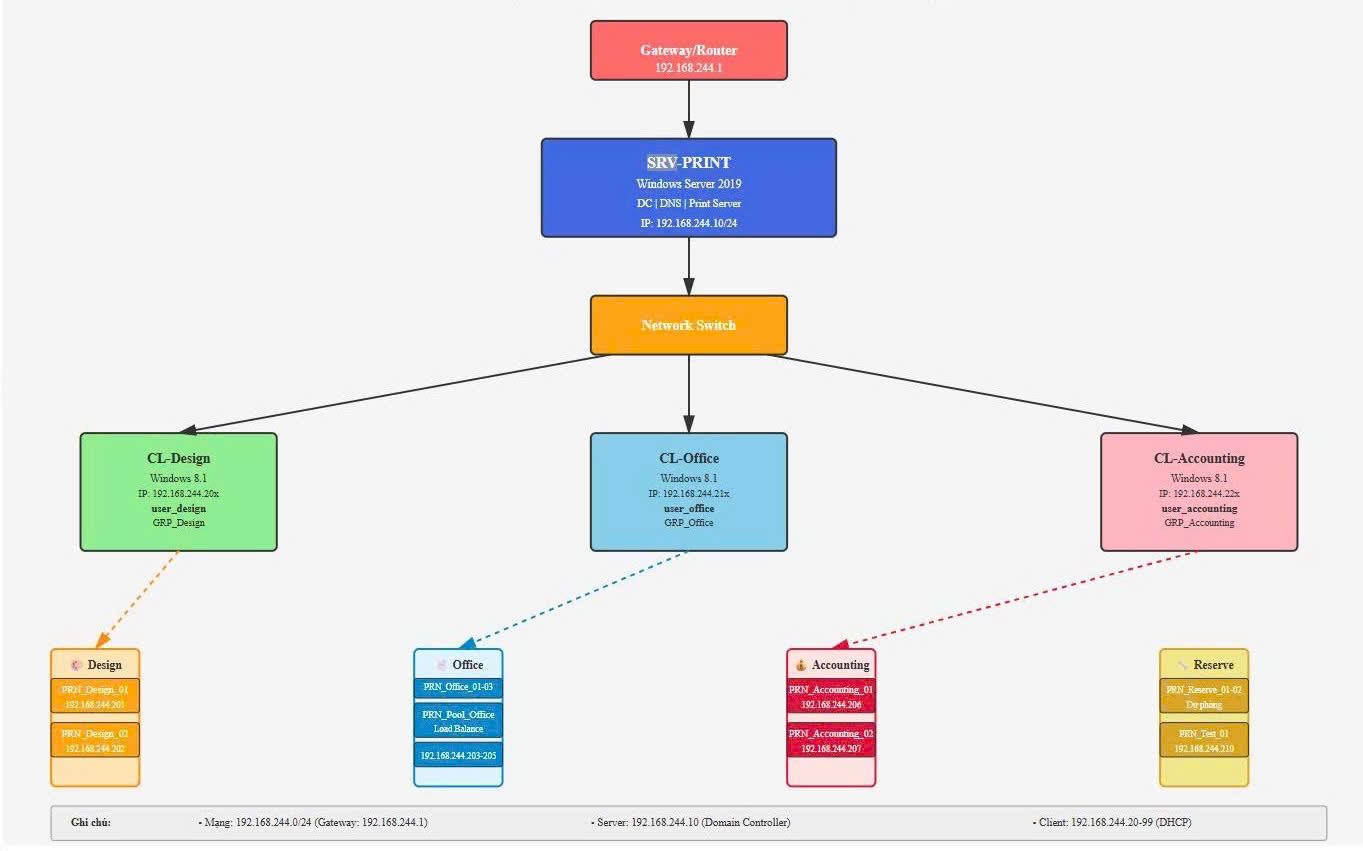
\includegraphics[width=0.85\linewidth]{img/d.jpg}
            \caption{Sơ đồ hoạt động của hệ thống Printer Server}
        \end{figure}
    \end{frame}
    
    \begin{frame}{Cấu trúc Active Directory}
        \begin{columns}[T]
            \begin{column}{0.48\textwidth}
                \textbf{Cấu trúc OU và Group:}
                \begin{itemize}
                    \item \textbf{ABC.local} (Forest)
                        \begin{itemize}
                            \item OU = Phong\_Thiet\_Ke
                                \begin{itemize}
                                    \item GRP\_Design\_Users
                                    \item user\_design
                                \end{itemize}
                            \item OU = Phong\_Van\_Phong
                                \begin{itemize}
                                    \item GRP\_Office\_Users
                                    \item user\_office
                                \end{itemize}
                            \item OU = Phong\_Ke\_Toan
                                \begin{itemize}
                                    \item GRP\_Accounting\_Users
                                    \item user\_accounting
                                \end{itemize}
                        \end{itemize}
                \end{itemize}
            \end{column}
            \begin{column}{0.3\textwidth}
                \begin{figure}
                    \centering
                    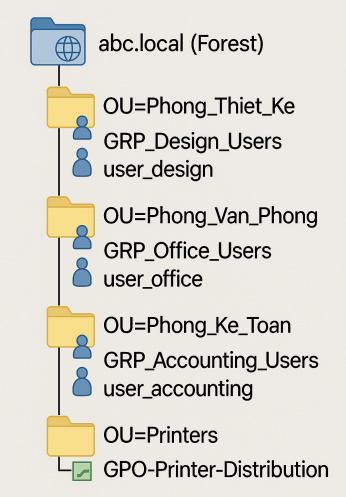
\includegraphics[width=\linewidth]{img/e.png}
                    \caption{Cấu trúc AD}
                \end{figure}
            \end{column}
        \end{columns}
    \end{frame}
    
    \begin{frame}{Phân bổ dải IP}
        \begin{table}[ht]
            \centering
            \small
            \begin{tabular}{|l|l|l|}
            \hline
            \textbf{Loại thiết bị} & \textbf{Dải IP} & \textbf{Số lượng} \\
            \hline
            Server & 192.168.244.10 & 1 \\
            \hline
            Gateway & 192.168.244.1 & 1 \\
            \hline
            Client computers & 192.168.244.20-99 & Tùy biến \\
            \hline
            Máy in vật lý/ảo & 192.168.244.201-210 & 10 \\
            \hline
            \end{tabular}
        \end{table}
        
        \vspace{0.3cm}
        \textbf{Thông tin Subnet:}
        \begin{itemize}
            \item Subnet Mask: 255.255.255.0 (/24)
            \item Network Address: 192.168.244.0
            \item Broadcast: 192.168.244.255
            \item Số IP khả dụng: 254 địa chỉ
        \end{itemize}
    \end{frame}

    % ===== CÁC BƯỚC TRIỂN KHAI =====
    \section{Triển khai hệ thống}
    \begin{frame}{Bước 1: Thiết lập Hostname và IP tĩnh}
        \textbf{Cấu hình cơ bản trên Server:}
        \begin{itemize}
            \item Đổi tên máy chủ thành SRV-PRINT
            \item Thiết lập IP tĩnh: 192.168.244.10/24
            \item Gateway: 192.168.244.1
            \item DNS: 8.8.8.8, 8.8.4.4 (tạm thời)
        \end{itemize}
        
        \vspace{0.3cm}
        \textbf{Công cụ sử dụng:}
        \begin{itemize}
            \item PowerShell cmdlets: Rename-Computer
            \item New-NetIPAddress
            \item Set-DnsClientServerAddress
        \end{itemize}
    \end{frame}
    
    \begin{frame}{Bước 2: Cài đặt vai trò Server}
        \textbf{Các vai trò cần cài đặt:}
        \begin{enumerate}
            \item \textbf{Print Server Role}
                \begin{itemize}
                    \item Install-WindowsFeature -Name Print-Server
                    \item Khởi động dịch vụ Print Spooler
                \end{itemize}
            \item \textbf{Active Directory Domain Services}
                \begin{itemize}
                    \item Install-WindowsFeature -Name AD-Domain-Services
                    \item Tạo Forest và Domain: ABC.local
                \end{itemize}
            \item \textbf{DNS Server}
                \begin{itemize}
                    \item Install-WindowsFeature -Name DNS
                    \item Tự động cấu hình khi tạo Domain
                \end{itemize}
        \end{enumerate}
    \end{frame}
    
    \begin{frame}{Bước 3: Tạo cấu trúc Active Directory}
        \textbf{Tạo Organizational Units (OU):}
        \begin{itemize}
            \item OU cho từng phòng ban
            \item OU cho máy in
            \item OU cho người dùng
        \end{itemize}
        
        \vspace{0.3cm}
        \textbf{Tạo Security Groups:}
        \begin{itemize}
            \item GRP\_Design\_Users
            \item GRP\_Office\_Users
            \item GRP\_Accounting\_Users
        \end{itemize}
        
        \vspace{0.3cm}
        \textbf{Tạo User Accounts:}
        \begin{itemize}
            \item user\_design, user\_office, user\_accounting
            \item Password: Manh31102005
            \item Thêm user vào nhóm tương ứng
        \end{itemize}
    \end{frame}

    % ===== TRIỂN KHAI MÁY IN =====
    \section{Triển khai máy in}
    \begin{frame}{Bước 4: Tạo TCP/IP Port}
        \textbf{Tạo 10 cổng TCP/IP cho máy in:}
        \begin{itemize}
            \item Dải IP: 192.168.244.201 – 192.168.244.210
            \item Port Name: IP\_192.168.244.201 – IP\_192.168.244.210
            \item Protocol: TCP Port 9100 (JetDirect)
        \end{itemize}
        
        \vspace{0.3cm}
        \textbf{Lệnh PowerShell:}
        \begin{itemize}
            \item Add-PrinterPort -Name [PortName]
            \item PrinterHostAddress [IP Address]
        \end{itemize}
    \end{frame}
    
    \begin{frame}{Bước 5: Cài đặt Driver}
        \textbf{Driver sử dụng:}
        \begin{itemize}
            \item HP Universal Print Driver PCL6 64-bit
            \item Lý do chọn:
                \begin{itemize}
                    \item Tương thích với nhiều model HP
                    \item Hỗ trợ môi trường doanh nghiệp
                    \item Dễ triển khai tự động
                \end{itemize}
        \end{itemize}
        
        \vspace{0.3cm}
        \textbf{Quy trình cài đặt:}
        \begin{enumerate}
            \item Dừng Print Spooler Service
            \item Cài driver bằng PNPUTIL
            \item Khởi động lại Print Spooler
            \item Kiểm tra driver đã cài thành công
        \end{enumerate}
    \end{frame}
    
    \begin{frame}{Bước 6: Tạo máy in theo phòng ban}
        \textbf{Danh sách máy in được tạo:}
        \begin{itemize}
            \item \textbf{Phòng Thiết kế:}
                \begin{itemize}
                    \item PRN\_Design\_01, PRN\_Design\_02
                \end{itemize}
            \item \textbf{Phòng Văn phòng:}
                \begin{itemize}
                    \item PRN\_Office\_01, PRN\_Office\_02, PRN\_Office\_03
                    \item PRN\_Pool\_Office (Printer Pool)
                \end{itemize}
            \item \textbf{Phòng Kế toán:}
                \begin{itemize}
                    \item PRN\_Accounting\_01, PRN\_Accounting\_02
                \end{itemize}
            \item \textbf{Máy in dự phòng:}
                \begin{itemize}
                    \item PRN\_Reserve\_01, PRN\_Reserve\_02, PRN\_Test\_01
                \end{itemize}
        \end{itemize}
        
        \vspace{0.2cm}
        \textbf{Tất cả máy in được chia sẻ (Shared = True)}
    \end{frame}
    
    \begin{frame}{Bước 7: Tạo Printer Pool}
        \textbf{Khái niệm Printer Pool:}
        \begin{itemize}
            \item Một máy in ảo quản lý nhiều máy in vật lý
            \item Tự động chia tải công việc in
            \item Tăng hiệu suất và độ tin cậy
        \end{itemize}
        
        \vspace{0.3cm}
        \textbf{Cấu hình PRN\_Pool\_Office:}
        \begin{itemize}
            \item Gồm 3 máy in vật lý:
                \begin{itemize}
                    \item PRN\_Office\_01 (192.168.244.203)
                    \item PRN\_Office\_02 (192.168.244.204)
                    \item PRN\_Office\_03 (192.168.244.205)
                \end{itemize}
            \item Tất cả 3 phòng ban đều có quyền sử dụng
            \item Priority: 30 (trung bình)
        \end{itemize}
    \end{frame}

    % ===== PHÂN QUYỀN =====
    \section{Phân quyền và kiểm soát}
    \begin{frame}{Phân quyền máy in bằng ICACLS}
        \textbf{Mục tiêu:}
        \begin{itemize}
            \item Mỗi phòng ban chỉ truy cập đúng máy in của mình
            \item Sử dụng ICACLS để phân quyền NTFS
        \end{itemize}
        
        \vspace{0.3cm}
        \textbf{Cấu hình phân quyền:}
        \begin{table}[ht]
            \centering
            \small
            \begin{tabular}{|l|l|}
            \hline
            \textbf{Máy in} & \textbf{Nhóm được cấp quyền} \\
            \hline
            PRN\_Design\_01/02 & GRP\_Design\_Users \\
            \hline
            PRN\_Office\_01/02/03 & GRP\_Office\_Users \\
            \hline
            PRN\_Accounting\_01/02 & GRP\_Accounting\_Users \\
            \hline
            PRN\_Pool\_Office & Cả 3 nhóm phòng ban \\
            \hline
            \end{tabular}
        \end{table}
        
        \vspace{0.2cm}
        \textbf{Quyền cấp:} (OI)(CI)(F) - Full Control
    \end{frame}
    
    \begin{frame}{Thiết lập độ ưu tiên (Priority)}
        \textbf{Nguyên tắc:}
        \begin{itemize}
            \item Số càng cao, độ ưu tiên càng lớn
            \item Range: 1 - 99
        \end{itemize}
        
        \vspace{0.3cm}
        \textbf{Cấu hình Priority:}
        \begin{table}[ht]
            \centering
            \small
            \begin{tabular}{|l|c|l|}
            \hline
            \textbf{Máy in} & \textbf{Priority} & \textbf{Lý do} \\
            \hline
            PRN\_Accounting\_01/02 & 75 & Bảo mật cao \\
            \hline
            PRN\_Design\_01/02 & 50 & Tốc độ quan trọng \\
            \hline
            PRN\_Pool\_Office & 30 & Chia sẻ chung \\
            \hline
            PRN\_Office\_01/02/03 & 25 & Tiêu chuẩn \\
            \hline
            \end{tabular}
        \end{table}
        
        \vspace{0.2cm}
        \textbf{Kết quả:} Máy in kế toán luôn được xử lý trước khi có nhiều job đồng thời
    \end{frame}
    \begin{frame}{Độ ưu tiên}
        \begin{figure}
            \centering
            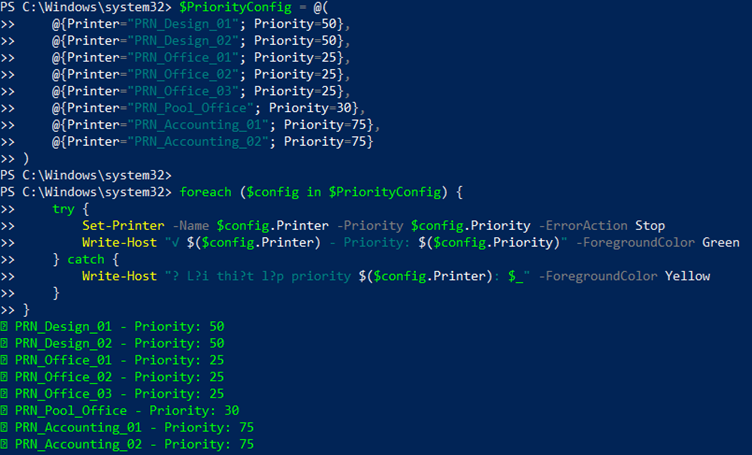
\includegraphics[width=0.85\linewidth]{img/s.png}
            \caption{Danh sách độ ưu tiên}
        \end{figure}
    \end{frame}

    % ===== PHÂN PHỐI TỰ ĐỘNG =====
    \section{Phân phối máy in qua GPO}
    \begin{frame}{Tạo Logon Script}
        \textbf{Mục đích:}
        \begin{itemize}
            \item Tự động kết nối máy in khi user đăng nhập
            \item Dựa trên Group Membership của user
        \end{itemize}
        
        \vspace{0.3cm}
        \textbf{Cơ chế hoạt động:}
        \begin{enumerate}
            \item Script đọc nhóm AD của user hiện tại
            \item Xác định user thuộc phòng ban nào
            \item Map máy in tương ứng với phòng ban đó
            \item Hiển thị danh sách máy in đã kết nối
        \end{enumerate}
        
        \vspace{0.3cm}
        \textbf{Công nghệ:}
        \begin{itemize}
            \item PowerShell Script (.ps1)
            \item .NET WindowsIdentity API
            \item Không cần AD Module trên Client
        \end{itemize}
    \end{frame}
    
    \begin{frame}{Gán Script qua GPO}
        \textbf{Các bước thực hiện:}
        \begin{enumerate}
            \item Tạo script: Map-DeptPrinters.ps1
            \item Lưu vào SYSVOL: 
                \begin{itemize}
                    \item \textbackslash\textbackslash SRV-PRINT\textbackslash sysvol\textbackslash ABC.local\textbackslash scripts
                \end{itemize}
            \item Tạo GPO: GPO\_PrinterDeploy
            \item Link GPO đến OU Users
            \item Cấu hình Logon Script trong GPO
        \end{enumerate}
        
        \vspace{0.3cm}
        \textbf{Kết quả:}
        \begin{itemize}
            \item Client tự động nhận máy in khi join domain
            \item Không cần cấu hình thủ công trên từng máy
            \item Dễ dàng mở rộng khi thêm user mới
        \end{itemize}
    \end{frame}
    \begin{frame}{Gán Script qua GPO}
    \centering
    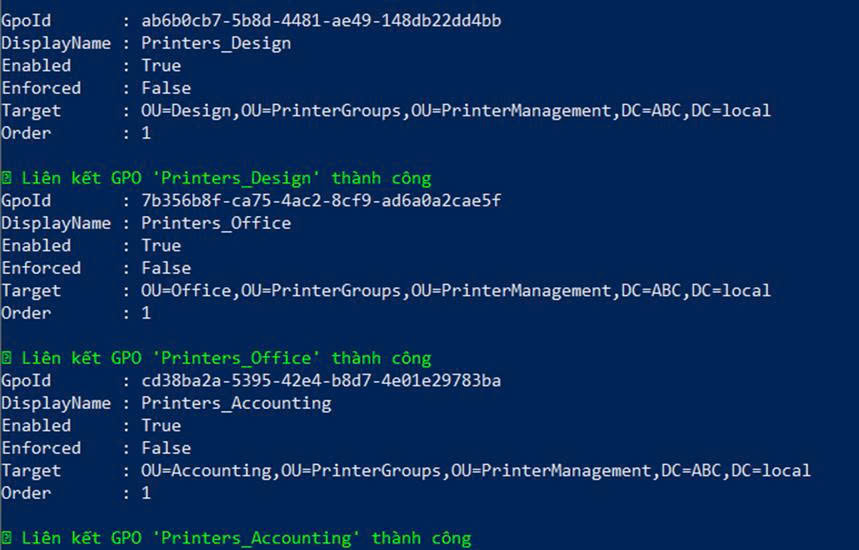
\includegraphics[width=0.75\textwidth]{img/o.jpg}
    
    \vspace{0.5cm} % Khoảng cách giữa 2 ảnh
    
    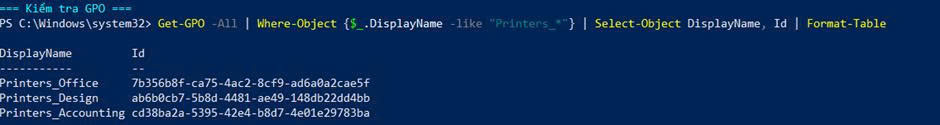
\includegraphics[width=0.75\textwidth]{img/p.jpg}
\end{frame}

    % ===== CẤU HÌNH CLIENT =====
    \section{Cấu hình Client}
    \begin{frame}{Join Domain và kiểm tra}
        \textbf{Bước 1: Join Domain}
        \begin{itemize}
            \item Cấu hình DNS trỏ về DC: 192.168.244.10
            \item Sử dụng Add-Computer cmdlet
            \item Restart máy sau khi join thành công
        \end{itemize}
        
        \vspace{0.3cm}
        \textbf{Bước 2: Đăng nhập với Domain Account}
        \begin{itemize}
            \item ABC\textbackslash user\_office
            \item ABC\textbackslash user\_design
            \item ABC\textbackslash user\_accounting
            \item Password: Manh31102005
        \end{itemize}
        
        \vspace{0.3cm}
        \textbf{Bước 3: Kiểm tra máy in tự động}
        \begin{itemize}
            \item Chạy: Get-Printer | Format-Table
            \item Máy in đã được map đúng theo phòng ban
            \item Không thấy máy in của phòng khác
        \end{itemize}
    \end{frame}
    
    \begin{frame}{Test chức năng in}
        \textbf{Quy trình test:}
        \begin{enumerate}
            \item Mở Notepad, soạn nội dung test
            \item File → Print → Chọn máy in
            \item Nhấn Print
        \end{enumerate}
        
        \vspace{0.3cm}
        \textbf{Kiểm tra Print Job:}
        \begin{itemize}
            \item \textbf{Trên Client:}
                \begin{itemize}
                    \item Get-WmiObject Win32\_PrintJob
                    \item Xem JobID, Owner, Status
                \end{itemize}
            \item \textbf{Trên Server:}
                \begin{itemize}
                    \item Get-PrintJob -PrinterName [Tên máy in]
                    \item Kiểm tra Queue và trạng thái
                \end{itemize}
        \end{itemize}
        
        \vspace{0.3cm}
        \textbf{Kết quả:} In thành công, job được xử lý đúng thứ tự priority
    \end{frame}

    % ===== GIÁM SÁT VÀ BÁO CÁO =====
    \section{Giám sát và báo cáo}
    \begin{frame}{Hệ thống Logging}
        \textbf{Tạo Custom Event Log:}
        \begin{itemize}
            \item Log Name: Print Service Log
            \item Source: PrinterServer
            \item Event ID: 1000 (Print Job Submitted)
        \end{itemize}
        
        \vspace{0.3cm}
        \textbf{Thông tin được ghi log:}
        \begin{itemize}
            \item Timestamp (thời gian chính xác)
            \item Username (người thực hiện in)
            \item PrinterName (máy in sử dụng)
            \item DocumentName (tên tài liệu)
            \item PageCount (số trang)
            \item Status (trạng thái thành công/thất bại)
        \end{itemize}
        
        \vspace{0.3cm}
        \textbf{Lưu trữ:}
        \begin{itemize}
            \item Event Viewer Log (Windows)
            \item CSV file: C:\textbackslash PrintLogs\textbackslash PrintHistory.csv
        \end{itemize}
    \end{frame}
    
    \begin{frame}{Chức năng báo cáo}
        \textbf{1. Báo cáo theo User:}
        \begin{itemize}
            \item Export-UserPrinterHistory -Username [tên user]
            \item Xuất lịch sử in của từng nhân viên
            \item Format: CSV file
        \end{itemize}
        
        \vspace{0.3cm}
        \textbf{2. Báo cáo tổng hợp:}
        \begin{itemize}
            \item Export-MonthlyPrintReport
            \item Thống kê 30 ngày gần nhất
            \item Bao gồm: Tổng số job, tổng số trang, phân bố theo phòng ban
        \end{itemize}
        
        \vspace{0.3cm}
        \textbf{3. Báo cáo theo khoảng thời gian:}
        \begin{itemize}
            \item Get-PrinterUsageReport -StartDate -EndDate
            \item Linh hoạt chọn khoảng thời gian
            \item Tính toán trung bình pages/job
        \end{itemize}
    \end{frame}
    \begin{frame}{Chức năng báo cáo}
    \centering
    \begin{minipage}{0.48\textwidth}
        \centering
        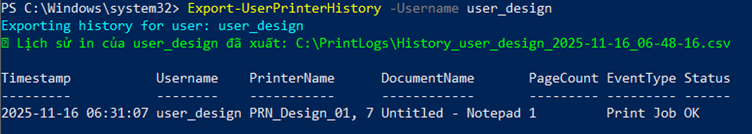
\includegraphics[width=\linewidth]{img/z.png}
        \captionof{Báo cáo theo user design}
    \end{minipage}
    \hfill
    \begin{minipage}{0.48\textwidth}
        \centering
        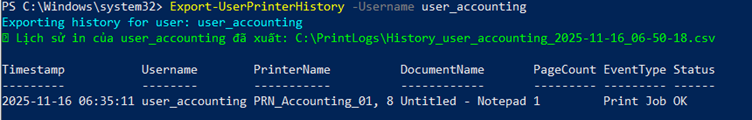
\includegraphics[width=\linewidth]{img/x.png}
        \captionof{Báo cáo theo user accounting}
    \end{minipage}
    
    \vspace{0.3cm}
    
    \begin{minipage}{0.48\textwidth}
        \centering
        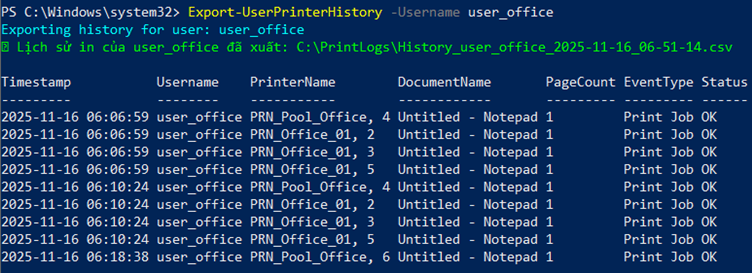
\includegraphics[width=\linewidth]{img/c.png}
        \captionof{Báo cáo theo user office}
    \end{minipage}
    \hfill
    \begin{minipage}{0.48\textwidth}
        \centering
        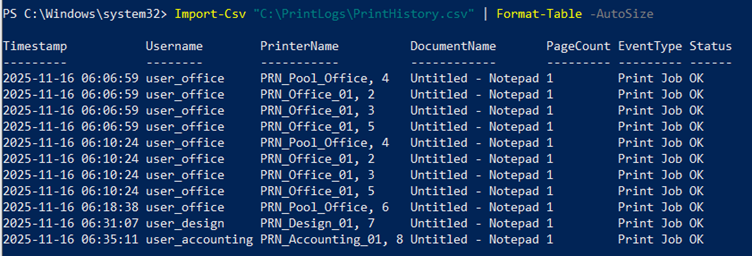
\includegraphics[width=\linewidth]{img/v.png}
        \captionof{Báo cáo 30 ngày}
    \end{minipage}
\end{frame}

    % ===== TROUBLESHOOTING =====
    \section{Troubleshooting}
    \begin{frame}{Công cụ xử lý sự cố}
        \textbf{Các function hỗ trợ:}
        \begin{enumerate}
            \item \textbf{Get-PrinterServerStatus}
                \begin{itemize}
                    \item Kiểm tra tổng quan hệ thống
                    \item Trạng thái các dịch vụ
                \end{itemize}
            \item \textbf{Clear-PrintQueue}
                \begin{itemize}
                    \item Xóa job bị treo
                    \item Hỗ trợ xóa theo máy in hoặc toàn bộ
                \end{itemize}
            \item \textbf{Test-PrinterConnection}
                \begin{itemize}
                    \item Kiểm tra kết nối đến máy in
                    \item Ping IP để xác định Online/Offline
                \end{itemize}
            \item \textbf{Restart-PrintSpooler}
                \begin{itemize}
                    \item Khởi động lại dịch vụ Print Spooler
                    \item Xử lý khi máy in không phản hồi
                \end{itemize}
        \end{enumerate}
    \end{frame}

    \begin{frame}{Các vấn đề thường gặp}
        \textbf{1. Client không nhận máy in:}
        \begin{itemize}
            \item Kiểm tra DNS trỏ đúng về DC
            \item Kiểm tra user có trong group đúng không
            \item Chạy gpupdate /force
        \end{itemize}
        
        \vspace{0.3cm}
        \textbf{2. Lỗi quyền truy cập:}
        \begin{itemize}
            \item Kiểm tra phân quyền bằng ICACLS
            \item Xác nhận user thuộc đúng nhóm AD
            \item Kiểm tra GPO có áp dụng đúng không
        \end{itemize}
        
        \vspace{0.3cm}
        \textbf{3. Job bị treo trong queue:}
        \begin{itemize}
            \item Sử dụng Clear-PrintQueue
            \item Restart Print Spooler nếu cần
            \item Kiểm tra log để tìm nguyên nhân
        \end{itemize}
    \end{frame}

    % ===== KẾT QUẢ KIỂM THỬ =====
    \section{Kết quả kiểm thử}
    \begin{frame}{Bảng tổng kết kiểm tra}
        \begin{table}[ht]
            \centering
            \tiny
            \begin{tabular}{|c|l|c|l|}
            \hline
            \textbf{STT} & \textbf{Chức năng} & \textbf{Kết quả} & \textbf{Ghi chú} \\
            \hline
            1 & Cấu hình mạng và DNS & PASS & Kết nối ổn định \\
            \hline
            2 & Join Domain & PASS & Tất cả client join OK \\
            \hline
            3 & Phân phối máy in qua GPO & PASS & Đúng policy \\
            \hline
            4 & Chức năng in ấn & PASS & In thành công \\
            \hline
            5 & Print Queue Management & PASS & Thứ tự ưu tiên đúng \\
            \hline
            6 & Event Logging & PASS & Event ID 307 đầy đủ \\
            \hline
            7 & Báo cáo theo User & PASS & CSV xuất chính xác \\
            \hline
            8 & Báo cáo 30 ngày & PASS & Tổng hợp đầy đủ \\
            \hline
            9 & Monitoring \& Status & PASS & Hiển thị real-time \\
            \hline
            10 & Troubleshooting Tools & PASS & Tất cả hoạt động \\
            \hline
            \end{tabular}
        \end{table}
    \end{frame}

    \begin{frame}{Demo kết quả}
        \textbf{Các kịch bản đã test:}
        \begin{enumerate}
            \item \textbf{User từ 3 phòng ban khác nhau đăng nhập}
                \begin{itemize}
                    \item Mỗi user chỉ thấy máy in của phòng mình
                    \item Máy in Pool hiển thị cho tất cả
                \end{itemize}
            \item \textbf{Test in đồng thời từ 3 client}
                \begin{itemize}
                    \item Job từ Accounting được xử lý trước (Priority 75)
                    \item Job từ Design xử lý tiếp theo (Priority 50)
                    \item Job từ Office xử lý cuối (Priority 25)
                \end{itemize}
            \item \textbf{Kiểm tra logging và báo cáo}
                \begin{itemize}
                    \item Event Log ghi đầy đủ thông tin
                    \item Báo cáo CSV xuất chính xác
                    \item Truy vết được lịch sử in của từng user
                \end{itemize}
        \end{enumerate}
    \end{frame}

    % ===== KẾT LUẬN =====
    \section{Kết luận}
    \begin{frame}{Kết quả đạt được}
        \textbf{Về kỹ thuật:}
        \begin{itemize}
            \item Triển khai hoàn toàn qua PowerShell CLI
            \item Tự động hóa 100\% quy trình cấu hình
            \item Phân quyền chính xác theo phòng ban
            \item Logging và audit đầy đủ
        \end{itemize}
        
        \vspace{0.3cm}
        \textbf{Về chức năng:}
        \begin{itemize}
            \item Printer Pool hoạt động ổn định
            \item Priority xử lý đúng thứ tự
            \item GPO phân phối máy in tự động
            \item Báo cáo thống kê chi tiết
        \end{itemize}
        
        \vspace{0.3cm}
        \textbf{Về vận hành:}
        \begin{itemize}
            \item Dễ dàng bảo trì và mở rộng
            \item Troubleshooting hiệu quả
            \item Giảm thiểu cấu hình thủ công
        \end{itemize}
    \end{frame}

    \begin{frame}{Giá trị doanh nghiệp}
        \textbf{Lợi ích mang lại:}
        \begin{itemize}
            \item \textbf{Tiết kiệm chi phí:}
                \begin{itemize}
                    \item Giảm thời gian cấu hình
                    \item Quản lý tập trung hiệu quả
                    \item Ít lỗi do thao tác thủ công
                \end{itemize}
            \item \textbf{Bảo mật cao:}
                \begin{itemize}
                    \item Phân quyền rõ ràng theo phòng ban
                    \item Audit trail đầy đủ
                    \item Truy vết được mọi hoạt động in
                \end{itemize}
            \item \textbf{Hiệu suất tốt:}
                \begin{itemize}
                    \item Printer Pool cân bằng tải
                    \item Priority đảm bảo công việc quan trọng
                    \item Giảm thiểu thời gian chờ đợi
                \end{itemize}
            \item \textbf{Dễ mở rộng:}
                \begin{itemize}
                    \item Thêm máy in mới dễ dàng
                    \item Thêm user/phòng ban nhanh chóng
                    \item Script có thể tái sử dụng
                \end{itemize}
        \end{itemize}
    \end{frame}

    \begin{frame}{Công nghệ sử dụng}
        \begin{table}[ht]
            \centering
            \small
            \begin{tabular}{|l|l|}
            \hline
            \textbf{Thành phần} & \textbf{Công nghệ} \\
            \hline
            Hệ điều hành Server & Windows Server 2019 Datacenter \\
            \hline
            Hệ điều hành Client & Windows 8.1 \\
            \hline
            Directory Service & Active Directory Domain Services \\
            \hline
            Print Service & Windows Print Server Role \\
            \hline
            Name Resolution & DNS Server \\
            \hline
            Automation & PowerShell 5.0+ \\
            \hline
            Group Policy & GPO - Logon Script \\
            \hline
            Permissions & ICACLS - NTFS ACL \\
            \hline
            Logging & Event Viewer + CSV \\
            \hline
            Virtualization & VMware Workstation Pro \\
            \hline
            \end{tabular}
        \end{table}
    \end{frame}

    \begin{frame}{Hướng phát triển}
        \textbf{Các cải tiến có thể thực hiện:}
        \begin{enumerate}
            \item \textbf{Tích hợp thêm tính năng:}
                \begin{itemize}
                    \item Email notification khi có lỗi
                    \item Web dashboard để giám sát
                    \item API để tích hợp với hệ thống khác
                \end{itemize}
            \item \textbf{Nâng cao bảo mật:}
                \begin{itemize}
                    \item Secure Print (PIN code)
                    \item Watermark tự động
                    \item Chặn in file nhạy cảm
                \end{itemize}
            \item \textbf{Tối ưu chi phí:}
                \begin{itemize}
                    \item Giới hạn số trang in
                    \item Báo cáo chi phí theo phòng ban
                    \item Cảnh báo khi vượt ngưỡng
                \end{itemize}
        \end{enumerate}
    \end{frame}


    % ===== PHỤ LỤC =====
    \section{Phụ lục}
    \begin{frame}{Danh sách lệnh PowerShell quan trọng}
        \begin{table}[ht]
            \centering
            \tiny
            \begin{tabular}{|l|l|}
            \hline
            \textbf{Lệnh} & \textbf{Chức năng} \\
            \hline
            Add-PrinterPort & Tạo port máy in \\
            \hline
            Add-Printer & Tạo máy in \\
            \hline
            Set-Printer & Sửa đặc tính máy in \\
            \hline
            Get-Printer & Liệt kê máy in \\
            \hline
            Get-PrintJob & Xem hàng đợi in \\
            \hline
            Remove-PrintJob & Xóa job \\
            \hline
            Restart-Service Spooler & Khởi động lại dịch vụ in \\
            \hline
            New-ADUser & Tạo user \\
            \hline
            New-ADGroup & Tạo group \\
            \hline
            Add-ADGroupMember & Thêm user vào group \\
            \hline
            Get-WinEvent & Truy vấn Event Log \\
            \hline
            icacls & Phân quyền NTFS \\
            \hline
            gpupdate /force & Cập nhật GPO \\
            \hline
            \end{tabular}
        \end{table}
    \end{frame}

    \begin{frame}{Port và Protocol}
        \begin{table}[ht]
            \centering
            \small
            \begin{tabular}{|c|c|l|}
            \hline
            \textbf{Port} & \textbf{Protocol} & \textbf{Dịch vụ} \\
            \hline
            9100 & TCP & JetDirect (Printer) \\
            \hline
            445 & TCP & SMB Sharing \\
            \hline
            139 & TCP/UDP & NetBIOS \\
            \hline
            53 & TCP/UDP & DNS \\
            \hline
            88 & TCP & Kerberos \\
            \hline
            389 & TCP/UDP & LDAP \\
            \hline
            \end{tabular}
        \end{table}
        
        \vspace{0.3cm}
    \end{frame}

    \begin{frame}{Tài liệu tham khảo}
        \textbf{Microsoft Documentation:}
        \begin{itemize}
            \item Microsoft Learn: Print Server Role
            \item Active Directory Best Practices
            \item PowerShell PrintManagement Module
            \item Group Policy Management Console Guide
        \end{itemize}
        
        \vspace{0.3cm}
        \textbf{Các nguồn khác:}
        \begin{itemize}
            \item HP Universal Print Driver Documentation
            \item Windows Server 2019 Administration Guide
            \item PowerShell Scripting Best Practices
            \item Network Printing Protocols (RFC 1179, RFC 3510)
        \end{itemize}
    \end{frame}

    % ===== KẾT THÚC =====
    \begin{frame}
        \begin{center}
            {\Huge \textbf{CẢM ƠN QUÝ THẦY CÔ}}
            
            \vspace{1cm}
            {\Large \textbf{VÀ CÁC BẠN ĐÃ LẮNG NGHE!}}
            
        \end{center}
    \end{frame}

\end{document}